\documentclass[11pt]{article}
\usepackage[top=1in, bottom=1in, left=1in, right=1in]{geometry}
\usepackage{float}
\usepackage{color}
\usepackage{picture}
\usepackage{listings}
\usepackage{verbatim}
\usepackage{caption}
\usepackage{makeidx}
\usepackage{graphicx}
\usepackage{amsmath}
\usepackage{subcaption}
\usepackage[utf8]{inputenc}
\usepackage[linktocpage=true]{hyperref}
\usepackage{multirow}
\usepackage{rotating}
\usepackage{lscape}
\makeatletter
\newcommand{\rmnum}[1]{\romannumeral #1}
\newcommand{\Rmnum}[1]{\expandafter\@slowromancap\romannumeral #1@}
\makeatother

% Used for the figures that have been inserted into the document.
\floatstyle{plain} 
\restylefloat{figure}

% Used so as not to indent paragraphs.
\setlength\parindent{0pt}

% Used for syntax highlighting in code.
\definecolor{skyblue}{rgb}{0.53, 0.81, 0.92}
\definecolor{lightred}{rgb}{0.90, 0.36, 0.36}
\definecolor{darkkhaki}{rgb}{0.71, 0.51, 0.06}

% Default parameters for listings package.
\lstset {
	tabsize=4,
	keywordstyle=\color{darkkhaki},
	commentstyle=\color{blue},
	showstringspaces=false,
	stringstyle=\color{lightred},
	frame=TLRB,
	captionpos=b,
	basicstyle=\small\ttfamily,
	breaklines=true
}

% Default parameters for hyperref package.
\hypersetup {
	pdftoolbar=true,
	pdfmenubar=true,
	colorlinks=true,
	linkcolor=red,
	citecolor=green,
	filecolor=magenta,
	urlcolor=cyan
}

\newcommand{\superscript}[1]{\ensuremath{^{\textrm{#1}}}}
\newcommand{\subscript}[1]{\ensuremath{_{\textrm{#1}}}}

\numberwithin{equation}{section}
%\setcounter{secnumdepth}{0}
\begin{document}

\begin{titlepage}

\begin{center}

\textsc{\LARGE Networks Assignment-4}\\[2.5cm]

\linethickness{0.5mm}
\line(1, 0){1\linewidth} \\[0.2cm]
{\huge \bfseries Packet Capturing Using Wireshark } \\[0.4cm]
\line(1, 0){1\linewidth} \\[2.5cm]

\begin{minipage}[t]{0.4\textwidth}
	\begin{flushleft} \large
	\emph{Prepared by:} \\[0.3cm]
	Nikhil Agarwal \\
	{\small 11012323} \\[0.2cm]
	Himanshu Upreti \\
	{\small 11012315} \\[0.2cm]
	\end{flushleft}
\end{minipage}
\begin{minipage}[t]{0.4\textwidth}
	\begin{flushright} \large
	\emph{Instructors:} \\[0.3cm]
	Dr. Sukumar Nandi\\[0.2cm]
	T. Venkatesh\\
	\end{flushright}
\end{minipage}

\vfill

% Bottom of the page
{\large \today}

\end{center}

\end{titlepage}

%\pagebreak

\renewcommand\contentsname{{\Huge Contents}\vspace{0.5cm}}
\addtocontents{toc}{~\hfill\textbf{Page}\par}
\cleardoublepage
\phantomsection
\addtocontents{toc}{\linespread{1.5}\selectfont}
\addcontentsline{toc}{section}{Contents}
\setcounter{tocdepth}{8}


\cleardoublepage
\phantomsection
%\addcontentsline{toc}{section}{List of Figures}
\renewcommand\listfigurename{{\Huge List of Figures}\vspace{0.5cm}}
\addtocontents{lof}{\linespread{1.5}\selectfont}
\addtocontents{lof}{~\hfill\textbf{Page}\par}
%\listoffigures

\pagebreak

\section*{PartA: Initials}

\textbf{1. Take a screenshot of this result. How many packets were transmitted from the IITG web server to your client in this? }\\
Ans: \textsc{44.}

\begin{figure}[H]
\begin{center}
		\centering
		\resizebox{1\linewidth}{!}{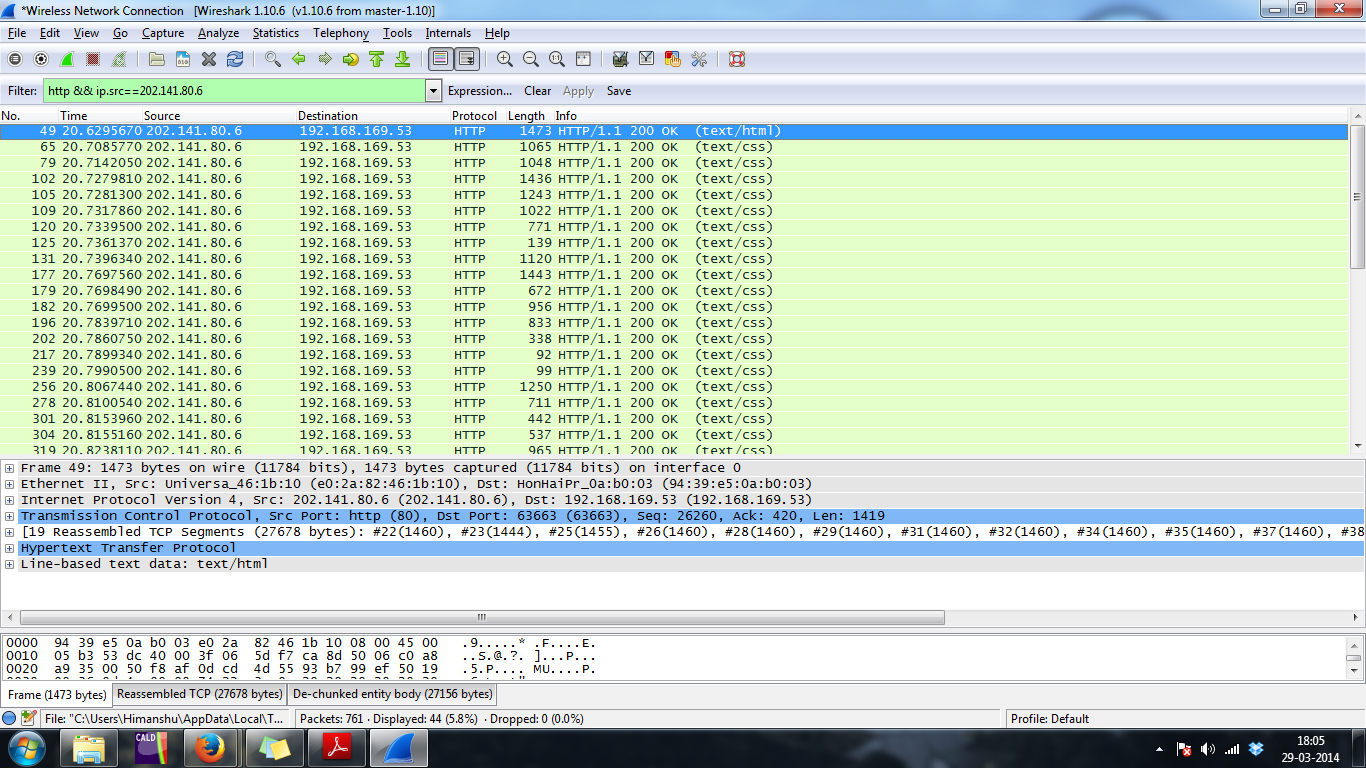
\includegraphics{parta}}
		\caption{ Packets transmitted from iitg web server}
		\label{fig:q1_f1_a}
\end{center}
\end{figure} 

\section*{PartB: HTTP} 
\subsection*{ The Basic HTTP GET/response Interaction}

\begin{figure}[H]
\begin{center}
		\centering
		\resizebox{1\linewidth}{!}{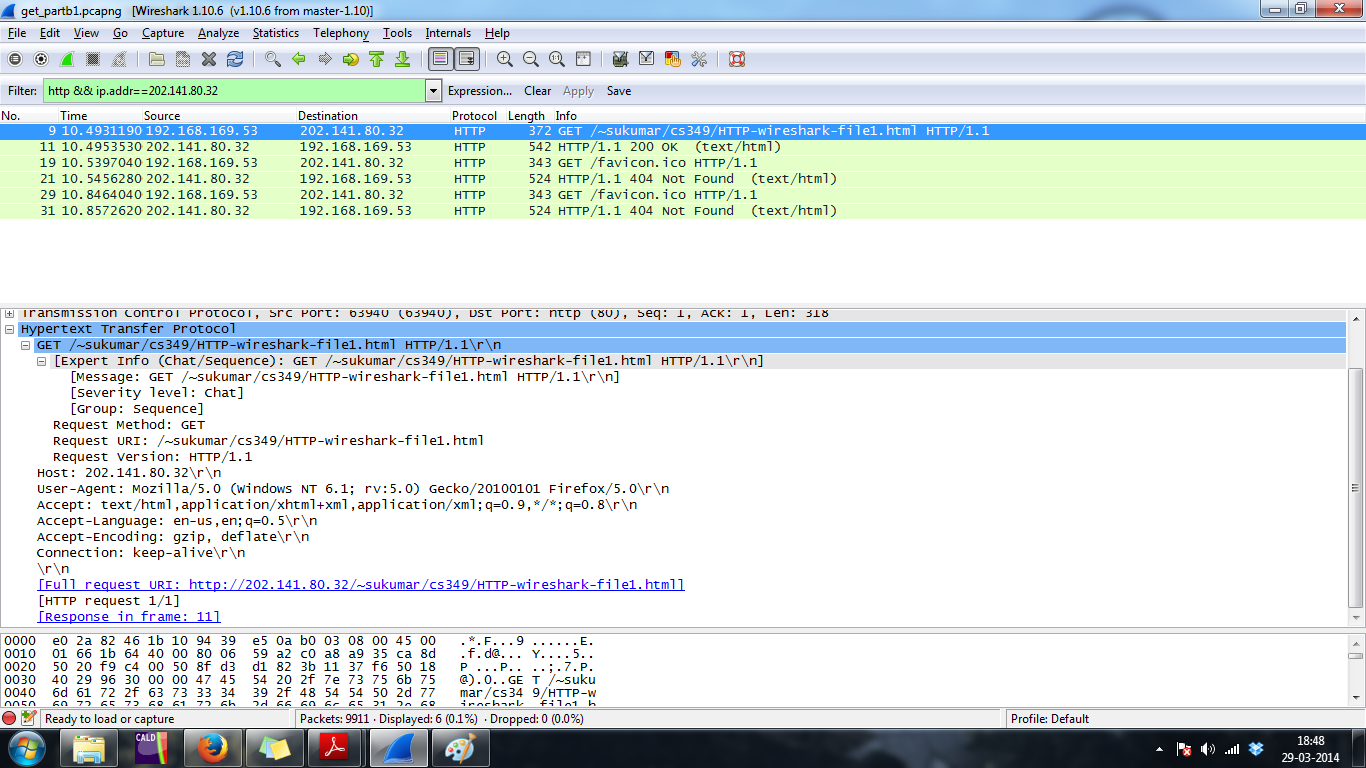
\includegraphics{partb_1_get}}
		\caption{Get message display}
		\label{fig:q1_f1_a}
\end{center}
\end{figure} 

\begin{figure}[H]
\begin{center}
		\centering
		\resizebox{1\linewidth}{!}{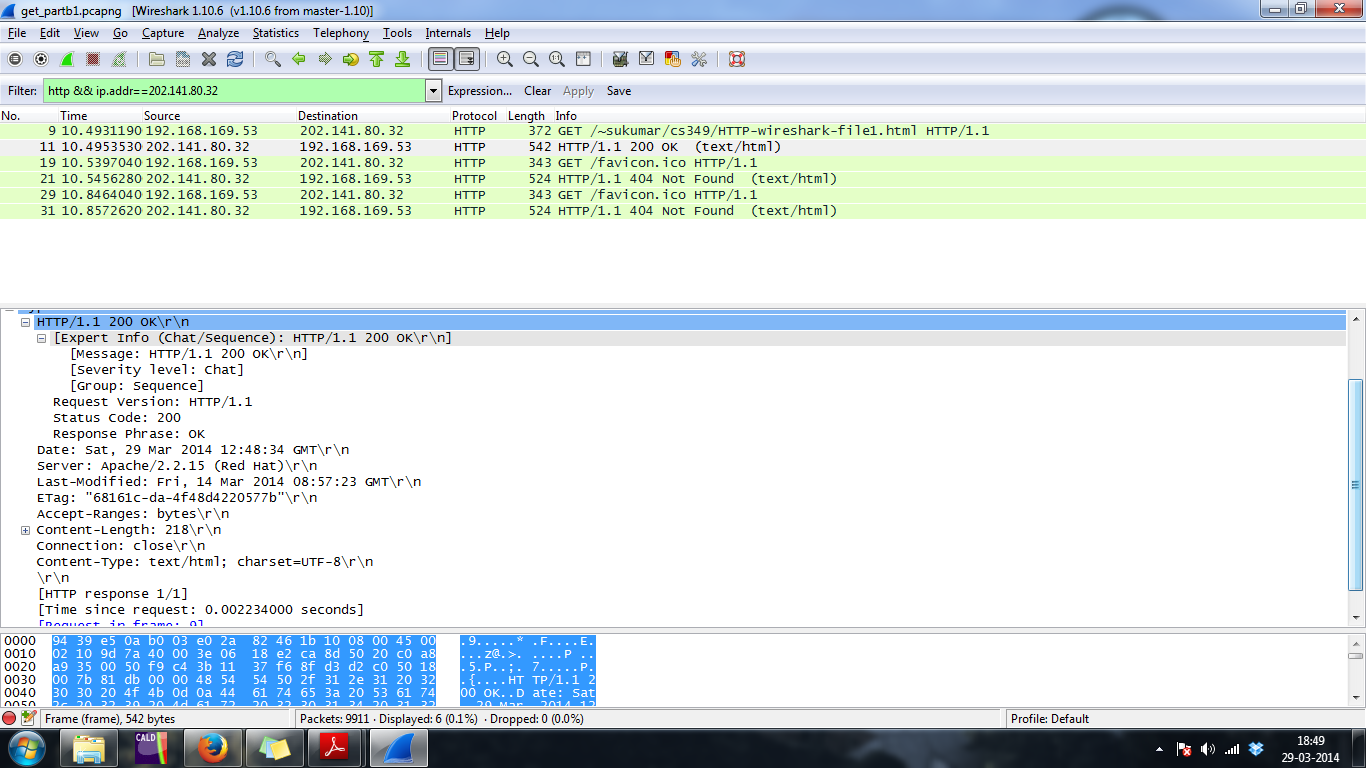
\includegraphics{partb_1_response}}
		\caption{Response message display}
		\label{fig:q1_f1_a}
\end{center}
\end{figure} 

\lstinputlisting[caption=\texttt{} HTTP GET/RESPONSE interaction, label=lst:q1_prog1, language=HTML]{partb_1.txt}

\textbf{Q1. Is your browser running HTTP version 1.0 or 1.1? What version of HTTP is the server running.} \\
Ans: \textsc{Both are running HTTP 1.1} \newline

\textbf{Q2. What languages (if any) does your browser indicate that it can accept to the server?} \\
Ans: \textsc{Accept-Language: en-us} \\

\textbf{Q3. What is the IP address of your computer?} \\
Ans: \textsc{The IP address of our computer is 192.168.169.53} \newline

\textbf{Q4. What is the status code returned from the server to your browser?} \\
\textsc{Ans: 200 OK (text/html)}  \newline

\textbf{Q5. When was the HTML file that you are retrieving last modified at the server?} \\
\textsc{Ans: Last-Modified: Fri , 14 Mar 2014 08:57:23 GMT} \newline

\textbf{Q6. How many bytes of content are being returned to your browser?} \\
\textsc{Ans: Content-Length: 218} \newline

\textbf{Q7. By inspecting the raw data in the packet content window, do you see any headers within the data that are not displayed in the packet-listing window? If so, name one.}\\
\textsc{Ans: No all of the headers can be found in the raw data.} \newline

\subsection*{The HTTP CONDITIONAL GET/response Interaction}

\begin{figure}[H]
\begin{center}
		\centering
		\resizebox{1\linewidth}{!}{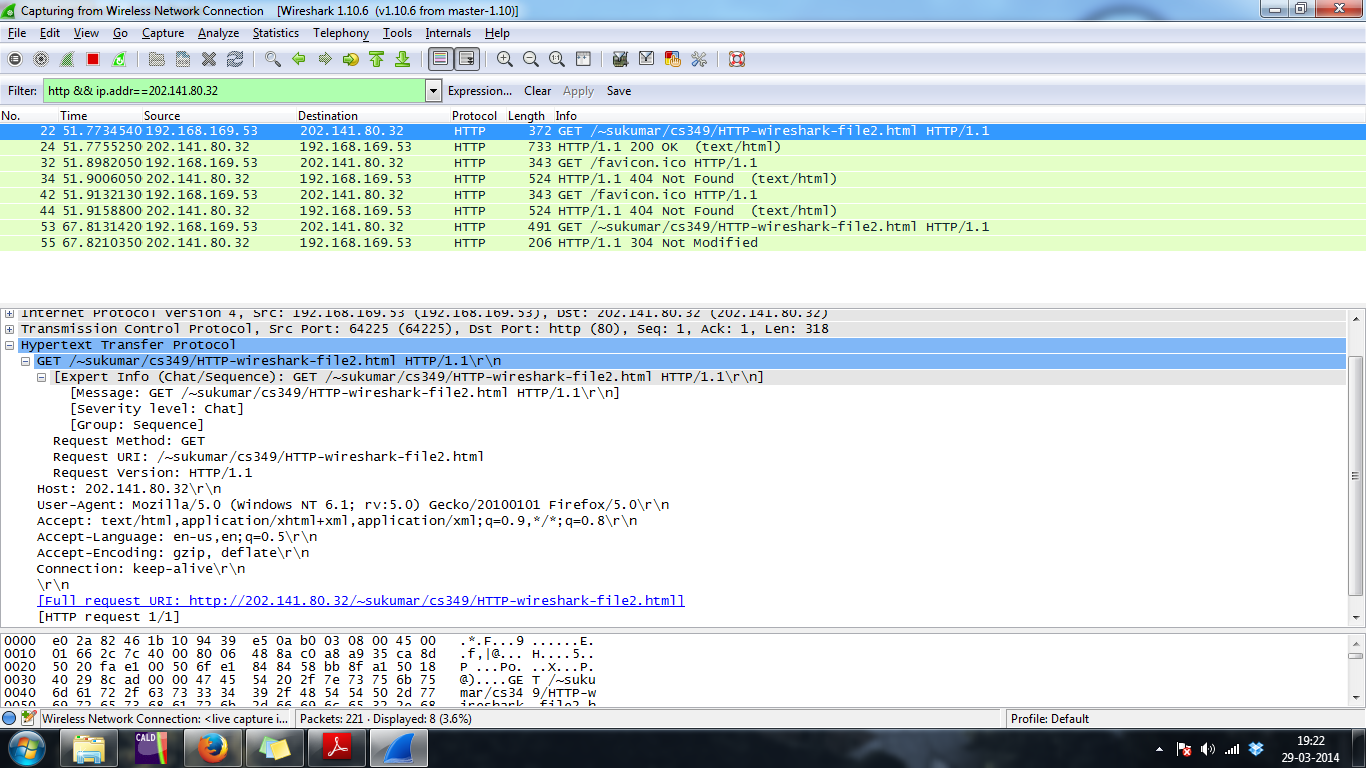
\includegraphics{parb_2_firstget}}
		\caption{First get message display}
		\label{fig:q1_f1_a}
\end{center}
\end{figure} 

\lstinputlisting[caption=\texttt{} HTTP CONDITIONAL GET/RESPONSE Interaction, label=lst:q1_prog1, language=HTML]{partb_2.txt}


\textbf{Q1. Inspect the contents of the first HTTP GET request from your browser to the server. Do you see an “IF-MODIFIED-SINCE” line in the HTTP GET?}

\textsl{Ans: No , we don't see an “IF-MODIFIED-SINCE” line in the HTTP GET as we are loading for first time ; so there is no question of modification.} \newline

\textbf{Q2. Inspect the contents of the server response. Did the server explicitly return the contents of the file? How can you tell?}

\textsl{Ans: Yes because we can see the contents in the "Line-based text data" field.}\newline

\textbf{Q3. Now inspect the contents of the second HTTP GET request from your browser to the server. Do you see an “IF-MODIFIED-SINCE:” line in the HTTP GET? If so, what information follows the “IF-MODIFIED-SINCE:” header?} 

\textsl{Ans: Yes. The information followed is: Fri, 14 Fri 2014 08:57:23 GMT which is the date of the last modification of the file from the previous GET request.}\newline

\textbf{Q4. What is the HTTP status code and phrase returned from the server in response to this second HTTP GET? Did the server explicitly return the contents of the file? Explain.} 

\textsl{Ans: The status code and phrase returned from the server is HTTP/1.1 304 Not Modified. The server didn’t explicitly return the contents of the file since the browser loaded it from its cache. (Also , the file was not modified since the first time we requested it)}
\subsection*{Retrieving Long Documents}

\begin{figure}[H]
\begin{center}
		\centering
		\resizebox{1\linewidth}{!}{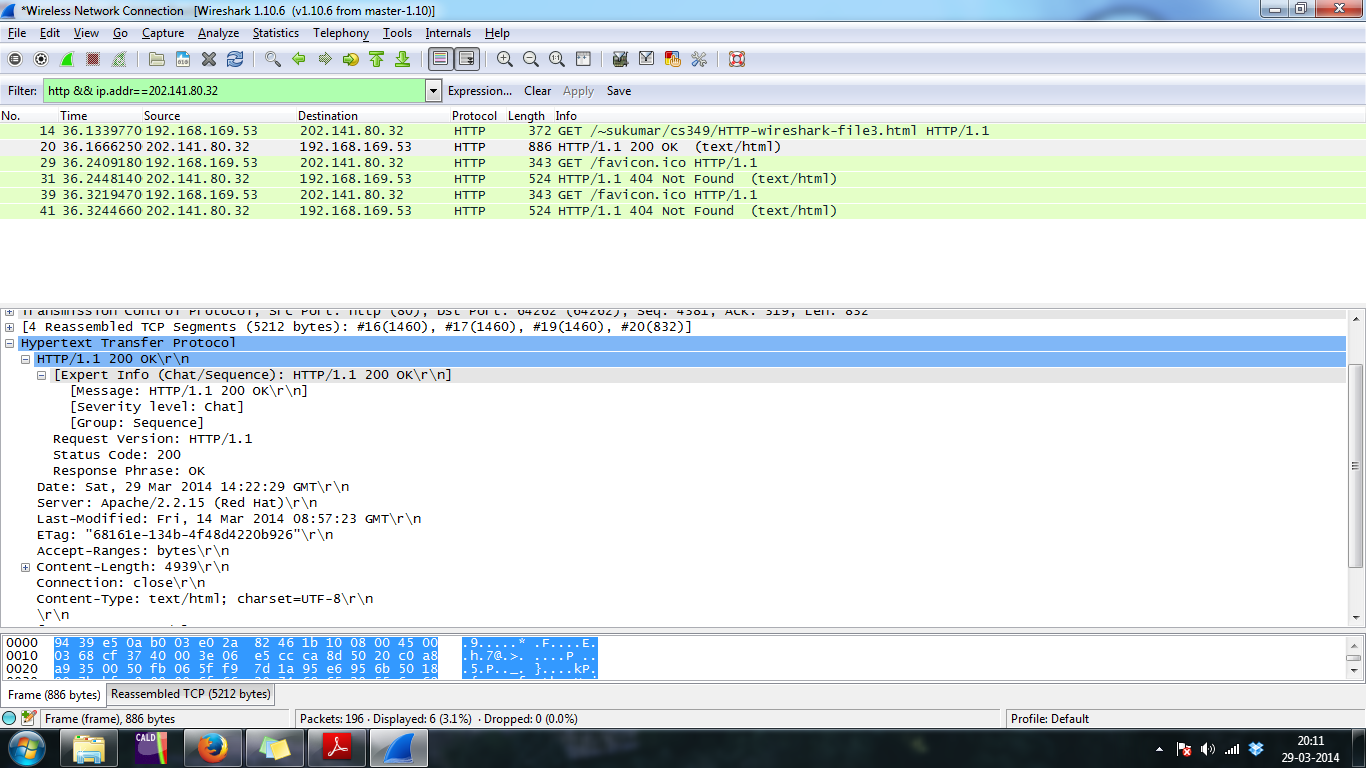
\includegraphics{partb_3_response}}
		\caption{response display}
		\label{fig:q1_f1_a}
\end{center}
\end{figure} 

\lstinputlisting[caption=\texttt{} HTTP Retrieving Long Documents, label=lst:q1_prog1, language=HTML]{partb_3.txt}

\textbf{Q1. How many HTTP GET request messages were sent by your browser?} 

\textsl{Ans: There was 1 HTTP GET request message sent by my browser.} \newline

\textbf{Q2. How many data-containing TCP segments were needed to carry the single HTTP response?} 

\textsl{Ans: There were 4 data containing TCP segments containing 1460 ,1460 ,1460 and 832 bytes respectively for a total of 5212 bytes.} \newline

\textbf{Q3. What is the status code and phrase associated with the response to the HTTP GET request?}

\textsl{Ans: The status code to the response is 200 OK, just like a single packet response.} \newline

\textbf{Q4. Are there any HTTP status lines in the transmitted data associated with a TCP-induced “Continuation”?}

\textsl{Ans: No, the transmitted data of TCP is only the content data.  The headers in the GET and OK request are the only two that indicate HTTP status lines.}

\section*{PARTC: UDP }

\begin{figure}[H]
\begin{center}
		\centering
		\resizebox{1\linewidth}{!}{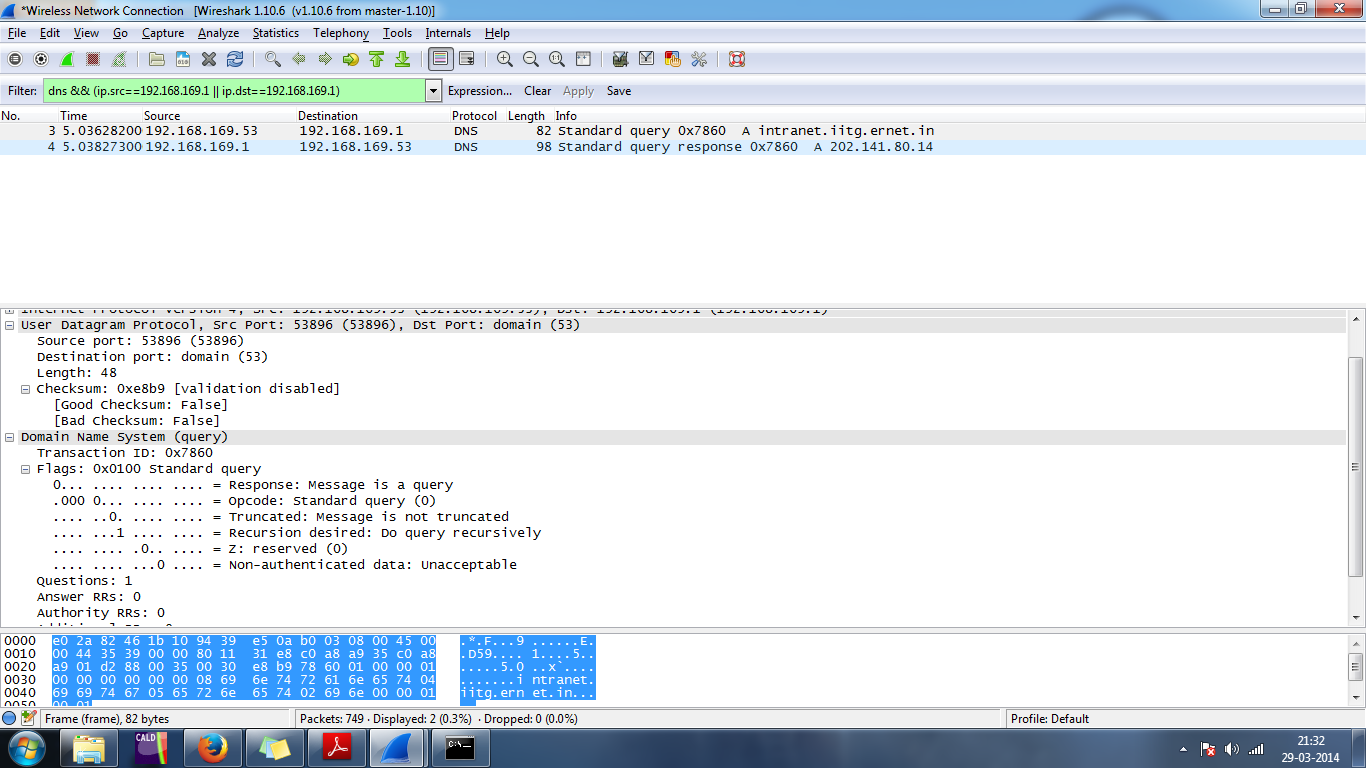
\includegraphics{partc}}
		\caption{UDP segment display}
		\label{fig:q1_f1_a}
\end{center}
\end{figure} 

\lstinputlisting[caption=\texttt{} UDP segments display, label=lst:q1_prog1, language=HTML]{partc.txt}

\textbf{a. Select one packet. From this packet, determine how many fields there are in the UDP header. Name these fields as they are named in the Wireshark display of segment fields.} 

\textsl{Ans: The UDP header contains 4 fields: source port, destination port, length, and checksum.} \newline

\textbf{b. What are the source and destination port numbers, in both decimal and hexadecimal format.} 

\textsl{Ans: Source Port : 53896 (0xd288)}  \\
             \hspace{5 cm} \textsl{Destination Port : 53(0x0035)} \\

\textbf{c. What is the value in the Length field in both decimal and hexadecimal format. What is the meaning of this value ?}

\textsl{Ans: The value in Length field is 48(0x30) \newline
              This value in the Length field defines the total length of user datagram (header plus data)} \newline

\textbf{d. What is the protocol number for UDP? Give your answer in both hexadecimal and decimal notation.} 

\textsl{Ans: The protocol number for UDP is 17 (0x11)} \newline

\textbf{e. Examine a pair of UDP packets in which the first packet is sent by your host and the second packet is a reply to the first packet. Describe the relationship between the port numbers in the two packets.}

\textsl{Ans: The source port of the UDP packet sent by the host is the same as the destination port of the reply packet, and conversely the destination port of the UDP packet sent by the host is the same as the source port of the reply packet.}

\section*{PARTD : TCP}

\begin{figure}[H]
\begin{center}
		\centering
		\resizebox{1\linewidth}{!}{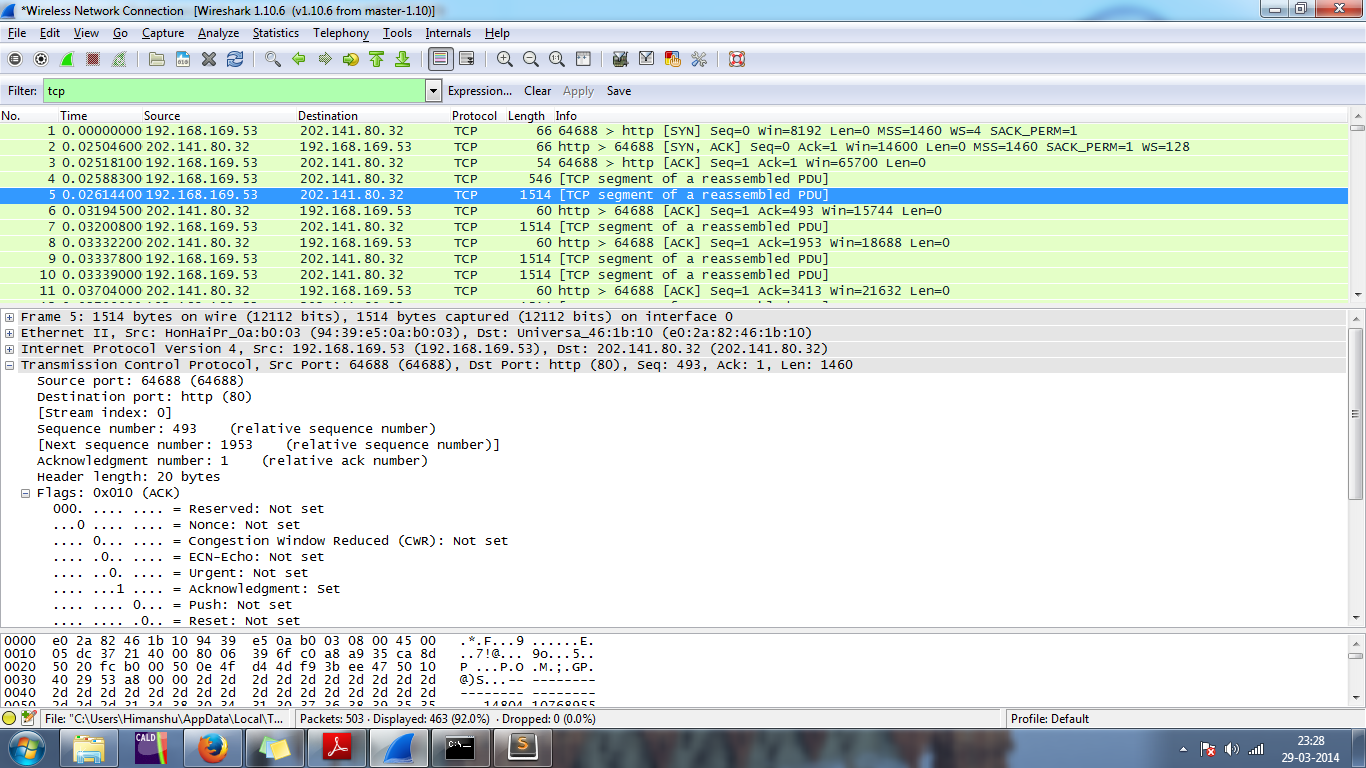
\includegraphics{partd_initial}}
		\caption{TCP first few segments}
		\label{fig:q1_f1_a}
\end{center}
\end{figure} 

\textbf{1. Print out a captured packet and indicate where you see the information that answers the following:} \newline

\textbf{a) What is the IP address and TCP port number used by your client computer (source) to transfer the file to 202.141.80.32? }

\textsl{Ans: IP address : 192.168.169.53 \\
Port number : 64688} \newline

\textbf{b) What is the IP address and TCP port number used by the server?} 

\textsl{IP address : 202.141.0.32 \\
Port number : 80 (http)} \newline

\textbf{2. Print out a captured packet and indicate where you see the information that answers the following:} \newline

\lstinputlisting[caption=\texttt{} TCP SYN segment, label=lst:q1_prog1, language=HTML]{partd_q2.txt}

\textbf{a) What is the sequence number of the TCP SYN segment that is used to initiate the TCP connection between the client computer and 202.141.80.32?}

\textsl{Ans: Sequence number of the TCP SYN segment is used to initiate the TCP connection between the client computer and 202.141.0.32. The value is 0 in this trace.} \newline

\textbf{b) What is it in the segment that identifies the segment as a SYN segment?} 

\textsl{Ans: The SYN flag is set to 1 and it indicates that this segment is a SYN segment. } \newline

\textbf{3. Print out a captured packet and indicate where you see the information that answers the following:} \newline

\lstinputlisting[caption=\texttt{} TCP SYNACK segment, label=lst:q1_prog1, language=HTML]{partd_q3.txt}

\textbf{a) What is the sequence number of the SYNACK segment sent by 202.141.80.32 to the client computer in reply to the SYN?} 

\textsl{Ans: Sequence number of the SYNACK segment from 202.141.80.32 to the client computer in reply to the SYN has the value of 0 in this trace.} \newline

\textbf{b) What is the value of the ACKnowledgement field in the SYNACK segment? }

\textsl{Ans: The value of the ACKnowledgement field in the SYNACK segment is 1.} \newline

\textbf{c) How did 202.141.80.32 server determine that value? }

\textsl{Ans: The value of the ACKnowledgement field in the SYNACK segment is determined by 202.141.80.32 by adding 1 to the initial sequence number of SYN segment from the client computer (i.e. the sequence number of the SYN segment initiated by the client computer is 0).} \newline

\textbf{ d) What is it in the segment that identifies the segment as a SYNACK segment? }

\textsl{Ans: The SYN flag and Acknowledgement flag in the segment are set to 1 and they indicate that this segment is a SYNACK segment.} \newline

\textbf{4. Print out a captured packet and indicate where you see the information that answers the following:} \newline

\lstinputlisting[caption=\texttt{} TCP first six segments, label=lst:q1_prog1, language=HTML]{partd_q4.txt}

\textbf{ What is the sequence number of the TCP segment containing the HTTP POST command? }

\textsl{Ans : Segment Number 4 is the TCP segment containing the HTTP POST command. The sequence number of this segment has the value of 1.} \newline

\textbf{Consider the TCP segment containing the HTTP POST as the first segment in the TCP connection.} \newline

\textbf{ a) What are the sequence numbers of the first six segments in the TCP connection (including the segment containing the HTTP POST)? At what time was each segment sent? }

\textsl{Ans: The HTTP POST segment is considered as the first segment. The  Segments 1 to 6 are Frame No. 4, 5, 7, 9, 10, and 12 in this trace respectively. The sequence numbers along with the time are tabulated below: }

\begin{table}[H]
\begin{center}
    \begin{tabular}{|p{2cm}|p{2cm}|p{2 cm}|p{2 cm}|}
    \hline
     Segment no & Frame no. & Sequence no.(Bytes) & Sent time\\ \hline
    1 & 4 & 1 & 0.025883\\ \hline
    2 & 5 & 493 & 0.02644\\ \hline
    3 & 7 & 1953 & 0.032008\\ \hline
    4 & 9 & 3413 & 0.033378\\ \hline
    5 & 10 & 4873 & 0.03339 \\ \hline
    6 & 12 & 6333 & 0.037099\\ \hline
    \end{tabular}
\end{center}
\end{table}


\textbf{ b) When was the ACK for each segment received? }

\textsl{Ans: The ACKs of segments 1 – 6 are No. 6, 8, 11, 14, 17, and 20 in this trace. Therefore , the corresponding values when they are received are tabulated below : } 

\begin{table}[H]
\begin{center}
    \begin{tabular}{|p{2cm}|p{2cm}|c|}
    \hline
     Segment no & Frame no. & Ack recvd time \\ \hline
    1 & 6 & 0.031945 \\ \hline
    2 & 8 & 0.033322 \\ \hline
    3 & 11 & 0.037040 \\ \hline
    4 & 14 & 0.044923 \\ \hline
    5 & 17 & 0.045843 \\ \hline
    6 & 20 & 0.046547 \\ \hline
    \end{tabular}
\end{center}
\end{table}


\textbf{ c) Do you see evidence of the use of cumulative ACKs in your trace? Explain.  }
 
\textsl{Ans: Yes we see evidence of the use of cumulative ACKs in our trace.  After the server sends an Ack for segment in frame 12, we receive 3 duplicate Acks for the next frame. Since the TCP follows faster retransmission mechanism so, my host sends the frame number 13 again. After receiving frame no. 13 , server directly sends an ACK for the segment in frame 16. Therefore , without acknowledging 13,14,15 it acknowledges the frame no. 16 and hence follow cumulative Acks. } \newline

\textbf{ d) Given the difference between when each TCP segment was sent, and when its acknowledgement was received, what is the RTT value for each of the six segments?  }

\textsl{Ans: The response time for each of them are tabulated below:}

\begin{table}[H]
\begin{center}
    \begin{tabular}{|p{2cm}|c|c|}
    \hline
    Sent time & Received time & RTT time\\ \hline
    
    0.025883 & 0.031945 & 0.006062\\ \hline
    0.02644 & 0.033322 & 0.007178  \\ \hline
    0.032008 & 0.037040 & 0.005032\\ \hline
    0.033378 & 0.044923 & 0.011545\\ \hline
    0.03339 & 0.045843 & 0.012453 \\ \hline
    0.037099 & 0.046547 & 0.009448\\ \hline
   
    \end{tabular}
\end{center}
\end{table}

\textbf{ e) What is the length of each of the first six TCP segments? }

\textsl{ Ans: Length of the first TCP segment (containing the HTTP POST): 446 bytes
Length of each of the other five TCP segments: 1514 bytes (MSS)}
\newline

\textbf{ f) What is the minimum amount of available buffer space advertised at the receiver for the entire trace? Does the lack of receiver buffer space ever throttle the sender? }

\textsl{Ans: The minimum amount of buffer space (receiver window) advertised at receiver for the entire trace is 14600 bytes, which shows in the first acknowledgement from the server. This receiver window grows steadily to 15744 for segment 6, 18688 for segment 8 and so on. The maximum window size the server advertises is 139136. Since at each packet acknowledgement server advertises more and more window size, the sender is never throttled. }\newline

\textbf{ g) Are there any retransmitted segments in the trace file? What did you check for (in the trace) in order to answer this question? How much data does the receiver typically acknowledge in an ACK? Can you identify cases where the receiver is ACKing every other received segment? Explain. }

\begin{figure}[H]
\begin{center}
		\centering
		\resizebox{1\linewidth}{!}{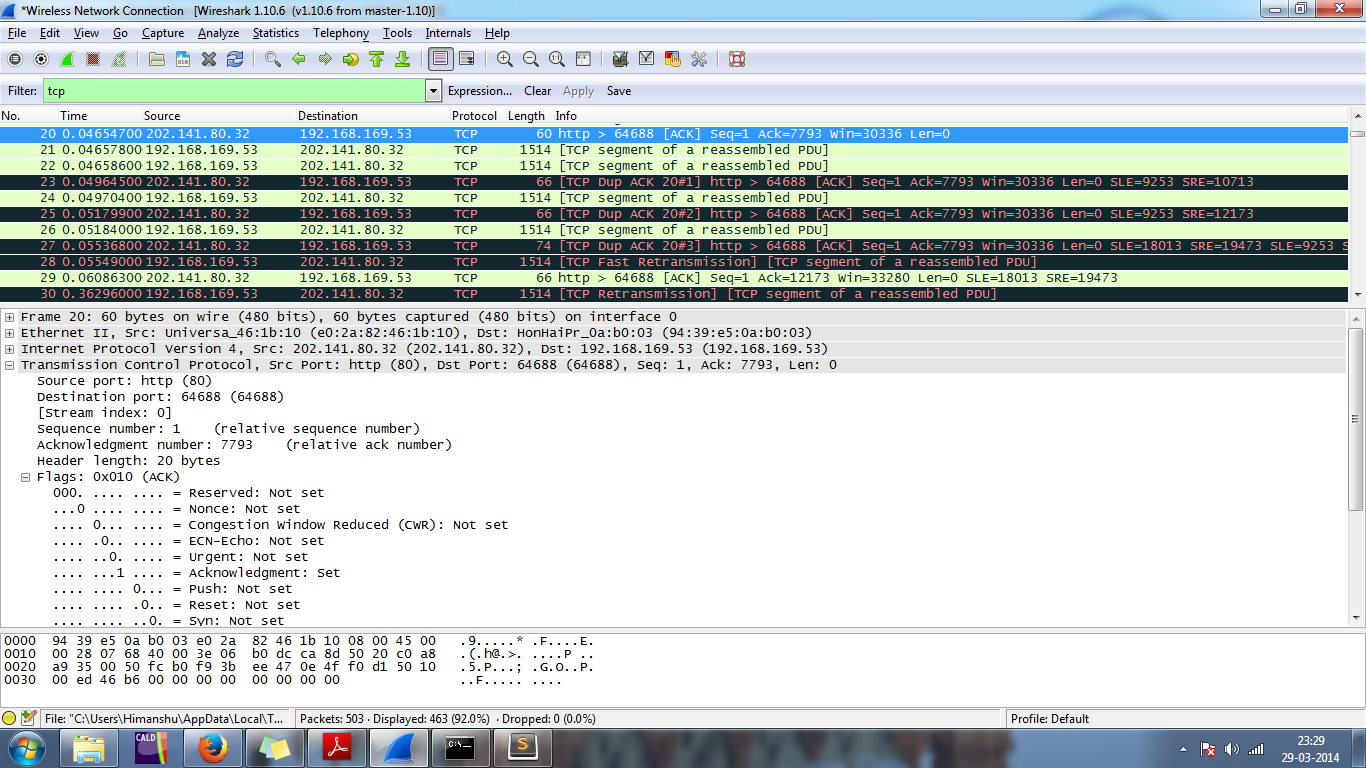
\includegraphics{partd_retransmitted}}
		\caption{TCP first few segments}
		\label{fig:q1_f1_a}
\end{center}
\end{figure}

\textsl{Ans: Yes, there are retransmitted packets in the trace file. We check for TCP Fast Retransmission Packet. Since, after receiving 3 Duplicate Acks, TCP retransmit the packet, I have to search for 3 Duplicate Acks or retransmitted packets. Frame no. 28 is a fast retransmission packet in our output. }

\begin{table}[H]
\begin{center}
    \begin{tabular}{|c|c|c|}
    \hline
    Ack Segment no. & Ack Sequence no. & Acknowledged Data\\ \hline
 
    1 & 493 & 493\\ \hline
    2 & 1953 & 1460  \\ \hline
    3 & 3413 & 1460\\ \hline
    4 & 4873 & 1460\\ \hline
    5 & 6333 & 1460 \\ \hline
    6 & 7793 & 1460\\ \hline
    7 & 7793 & 0\\ \hline  
    8 & 7793 & 0\\ \hline 
    9 & 7793 & 0\\ \hline
    10 & 12173 & 4380\\ \hline 
    11 & 13633 & 1460\\ \hline
    \end{tabular}
\end{center}
\end{table}

\textsl{ From the above table it is clear that receiver typically acknowledges 1460 bytes of data. In my case, receiver is never ACKing every other segment. From the above table, after fast retransmission, receiver ACKs $3*1460=4380$ bytes of data together and I searched through the whole file to find 2*1460=2920 bytes of data but I was not able to find it. From the above table receiver directly ACKS 4380 bytes of data due to cumulative ACK. }\newline



\end{document}